\documentclass[11pt,a4paper]{article}
\usepackage[T1]{fontenc}
\usepackage[utf8]{inputenc}
\usepackage{lmodern}
\usepackage{amsmath,amssymb,amsthm,mathtools,mathrsfs}
\usepackage{graphicx,float,xcolor,multicol}
\usepackage[shortlabels]{enumitem}
\usepackage[margin=27mm]{geometry}
\usepackage{microtype,needspace,placeins}
\usepackage{tikz,tikz-cd}
\usetikzlibrary{arrows.meta,calc,positioning,patterns,decorations.pathreplacing}
\usepackage[colorlinks=true,linkcolor=teal,urlcolor=teal,citecolor=teal]{hyperref}
\setlength{\parindent}{0pt}
\setlength{\parskip}{.6em}
\setcounter{secnumdepth}{0}
\allowdisplaybreaks
\raggedbottom
\providecommand{\cross}{\times}
\DeclareUnicodeCharacter{2020}{\ensuremath{\dagger}}
\DeclareMathOperator{\supp}{supp}
\DeclareMathOperator*{\esssup}{ess\,sup}
\providecommand{\chapter}{\section}
\newenvironment{tool}[2]{\subsection*{Tool #1 --- #2}}{}
\newcommand{\ToolRef}[1]{Tool #1}
\newcommand{\FigureTag}[2]{\textit{Figure #1}}
\newcommand{\Result}[1]{\subsection*{#1}}
\newcommand{\Application}[1]{\subsubsection*{Application\if\relax\detokenize{#1}\relax\else\space--- #1\fi}}
\newcommand{\ProofHeading}{\par\textit{Proof.}\space}
\newcommand{\ProofOf}[1]{\par\textit{Proof of #1.}\space}
\newcommand{\RemarkHeading}{\par\textbf{Remark.}\space}
\newcommand{\NoteHeading}{\par\textbf{Note.}\space}
\newcommand{\ExerciseHeading}{\par\textbf{Exercise.}\space}

% Rendering support only; mathematical text is in each independent post.
\usepackage{booktabs,array,longtable}
\definecolor{HandoutBlue}{HTML}{2F6690}
\definecolor{HandoutNavy}{HTML}{17365D}
\newtheorem{theorem}{Theorem}
\newtheorem{lemma}[theorem]{Lemma}
\newtheorem{proposition}[theorem]{Proposition}
\newtheorem{corollary}[theorem]{Corollary}
\newtheorem{conjecture}[theorem]{Conjecture}
\newtheorem{definition}{Definition}
\newtheorem{example}{Example}
\newtheorem{namedtoolcounter}{Tool}
\newenvironment{namedtool}[1]{\begin{namedtoolcounter}[#1]}{\end{namedtoolcounter}}
\newtheorem*{claim}{Claim}
\newtheorem*{remark}{Remark}
\newtheorem*{exercise}{Exercise}
\newtheorem*{question}{Question}
\newtheorem*{observation}{Observation}
\newcommand{\SourceChapter}[2]{\section*{#2}}
\newcommand{\Lecture}[2]{\section*{Lecture #1: #2}}
\newcommand{\unclear}[1]{\textit{[unclear: #1]}}
\newcommand{\sourcegap}{\textit{[unfinished in the source]}}
\DeclareMathOperator{\dist}{dist}
\DeclareMathOperator{\id}{id}
\DeclareMathOperator{\Hol}{Hol}
\DeclareMathOperator{\Per}{Per}
\DeclareMathOperator{\Fix}{Fix}
\DeclareMathOperator{\diam}{diam}
\DeclareMathOperator{\Var}{Var}
\DeclareMathOperator{\Leb}{Leb}
\DeclareMathOperator{\Hom}{Hom}
\DeclareMathOperator{\End}{End}
\DeclareMathOperator{\Ann}{Ann}
\DeclareMathOperator{\Spec}{Spec}
\DeclareMathOperator{\Max}{Max}
\DeclareMathOperator{\Ob}{Ob}
\DeclareMathOperator{\Tor}{Tor}
\DeclareMathOperator{\Ass}{Ass}
\DeclareMathOperator{\Mor}{Mor}
\DeclareMathOperator{\Fun}{Fun}
\DeclareMathOperator{\Nat}{Nat}
\DeclareMathOperator{\Cone}{Cone}
\DeclareMathOperator{\MCG}{MCG}
\DeclareMathOperator{\Aut}{Aut}
\DeclareMathOperator{\Deck}{Deck}
\DeclareMathOperator{\SL}{SL}
\DeclareMathOperator{\PSL}{PSL}
\DeclareMathOperator{\Area}{Area}
\DeclareMathOperator{\im}{im}
\DeclareMathOperator{\PSh}{PSh}
\newcommand{\CRing}{\mathsf{CRings}}
\newcommand{\AMod}{A\text{-}\mathsf{Mod}}
\newcommand{\Ab}{\mathsf{Ab}}
\newcommand{\Z}{\mathbb Z}
\newcommand{\Q}{\mathbb Q}
\newcommand{\R}{\mathbb R}
\newcommand{\C}{\mathbb C}
\newcommand{\N}{\mathbb N}
\newcommand{\kk}{\mathbb k}
\renewcommand{\aa}{\mathfrak a}
\newcommand{\bb}{\mathfrak b}
\newcommand{\pp}{\mathfrak p}
\newcommand{\qq}{\mathfrak q}
\newcommand{\mm}{\mathfrak m}
\newcommand{\nn}{\mathfrak n}
\newcommand{\rad}{\mathrm r}
\newcommand{\cat}[1]{\mathsf{#1}}
\setcounter{secnumdepth}{0}
\allowdisplaybreaks

\graphicspath{{figures/complex-dynamics-notes/}}
\begin{document}
\section*{Prime Ends and Landing of External Rays}
% BLOG-CONTENT-BEGIN
Recall the Riemann mapping theorem.
\setcounter{theorem}{32}\begin{theorem}[Riemann mapping theorem]
For a simply connected domain $U\subset\mathbb C$, there is a biholomorphism $\varphi\colon U\to\mathbb D$, unique after prescribing suitable initial values, namely $\varphi^{-1}(0)$ and $(\varphi^{-1})'(0)$.
\end{theorem}
Nothing in this theorem says that the map extends homeomorphically to $\overline U$. We first sketch Carath\'eodory's work on extension, then interpret it for a monic polynomial $f\colon\widehat{\mathbb C}\to\widehat{\mathbb C}$ of degree at least two, with $J=\partial K$ connected. Equivalently, $\mathcal A(\infty)$ contains no finite critical point of $f$.
\subsection{A sketch of Carath\'eodory's work}
Let $\varphi\colon U\to\mathbb D$ be a conformal isomorphism. For now we avoid hyperbolic geometry: the spherical metric $\rho(z)|dz|$ on $\widehat{\mathbb C}$ captures Carath\'eodory's strategy. Impose it on both $\mathbb D$ and $U$.
% Source page 2
For a square $I^2\subset\widehat{\mathbb C}$, its area is $\iint_{I^2}\rho(x+iy)^2\,dx\,dy$, and the length of a horizontal segment $y=C$ is $\int_I\rho(x+iC)\,dx$. Cauchy--Schwarz gives
\[
\left(\int_I\rho(x+iy)\,dx\right)^2
\le\left(\int_I1^2\,dx\right)\left(\int_I\rho(x+iy)^2\,dx\right).
\]
Hence $\int_I L(y)^2\,dy=O(\operatorname{Area}(I^2))$. Thinking of $I^2\cong\mathbb D$, we conclude that for almost every radial line $r\mapsto re^{i\theta}$, the limit $\lim_{r\to1}\varphi^{-1}(re^{i\theta})\in\partial U$ exists.
\begin{figure}[H]\centering
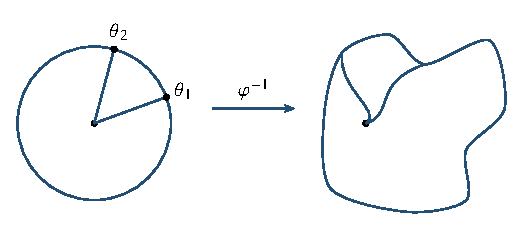
\includegraphics[width=.76\textwidth]{cd8-fig-01.pdf}
\FigureTag{CD8.1}{fig:cd8-01}
\end{figure}
For almost every $\theta\in(0,2\pi]$, this gives a candidate for $\varphi^{-1}(e^{i\theta})$. To ensure continuous extension to the boundary, every sequence $z_j\to e^{i\theta}$ must satisfy $\varphi^{-1}(z_j)\to\varphi^{-1}(e^{i\theta})$.

The idea is to divide $U$ by crosscuts $A\subset U$, with $A\cong(0,1)$, $\overline A\cong[0,1]$, and $|\partial A\cap\overline U|=2$.
% Source page 3
For example, a crosscut $A$ joins boundary points $x,y$. Since $U\cong\mathbb D$, every sequence $x_i\to\partial U$ has its image accumulating on $\partial\mathbb D$. Thus there is a homeomorphism $\widetilde\varphi\colon\overline U/\partial U\to\overline{\mathbb D}/\partial\mathbb D\cong S^2$.
\begin{figure}[H]\centering
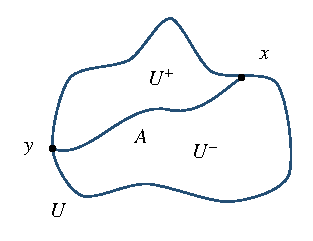
\includegraphics[width=.51\textwidth]{cd8-fig-02.pdf}
\FigureTag{CD8.2}{fig:cd8-02}
\end{figure}
Viewed in $S^2$, $A$ is a Jordan curve, so it divides $U$ into $U^+,U^-$, the signs depending on the orientation of $A$. These are called crosscut neighbourhoods.

To prevent failure of boundary continuity of $\varphi$ or $\varphi^{-1}$, build a lasso around boundary points: a fundamental chain $\mathcal N=\{N_j\}_j$ of crosscut neighbourhoods with $N_1\supset N_2\supset\cdots$. If $A_j$ are the corresponding crosscuts, require $\overline A_j\cap\overline A_i=\varnothing$ for $i\ne j$, and $\diam(\overline A_j)\to0$.
\begin{figure}[H]\centering
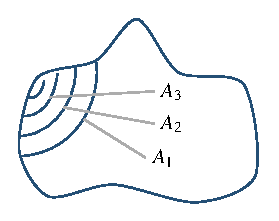
\includegraphics[width=.52\textwidth]{cd8-fig-03.pdf}
\FigureTag{CD8.3}{fig:cd8-03}
\end{figure}
\setcounter{theorem}{33}\begin{theorem}[Carath\'eodory]
A conformal isomorphism $\psi\colon\mathbb D\to U$ extends continuously onto $\widetilde\psi\colon\overline{\mathbb D}\to\overline U$ if and only if $\partial U$ is locally connected.
\end{theorem}
In our setting the conformal isomorphism is the B\"ottcher map $\phi\colon\mathbb C\setminus K\to\mathbb C\setminus\overline{\mathbb D}$. The sets $\{z:\arg\phi(z)=\theta\}$ are external rays, incident at angle $\theta$. For $\theta\in\mathbb R/\mathbb Z$, let $R_\theta=\{re^{2\pi i\theta}:r>1\}$ in the exterior disc. Set
\[
\gamma(t)=\lim_{r\to1}\phi^{-1}(re^{2\pi it}).
\]
If this exists, we say that $R_t$ lands at $\gamma(t)\in\partial K=J$. Let us translate Carath\'eodory's work into this setting.
% Source page 5
\setcounter{theorem}{34}\begin{theorem}[Landing criterion]\label{cd8:landing}
The following are equivalent:
\begin{itemize}
\item every ray $R_t$, $t\in\mathbb R/\mathbb Z$, lands, and $\gamma(t)$ is continuous;
\item $J=\partial K$ is locally connected;
\item $K$ is locally connected;
\item $\phi^{-1}\colon\mathbb C\setminus\overline{\mathbb D}\to\mathbb C\setminus K$ extends continuously to the boundary.
\end{itemize}
\end{theorem}
\begin{proof}
Immediate from Carath\'eodory's theorem.
\end{proof}
We offer a slightly deeper insight than the landing criterion.
\setcounter{theorem}{35}\begin{theorem}[Rational rays land]\label{cd8:rational-rays}
Every periodic rational ray $R_t$ lands at a repelling or parabolic periodic point, or an eventually periodic point.
\end{theorem}
% Source page 6
\setcounter{theorem}{37}\begin{lemma}[Preparatory lemma]\label{cd8:preparatory}
If $R_t=f(R_t)$ lands at $z_0$, then $z_0$ is a repelling or parabolic fixed point.
\end{lemma}
\begin{remark}
One can also prove the converse of Theorem~\href{https://codezen1729.github.io/math-blog/\#/post/prime-ends-and-landing-of-external-rays}{36}.
\end{remark}
% BLOG-CONTENT-END
\end{document}
